% !TeX program = pdflatex
\documentclass[11pt]{article}
\usepackage[margin=1in]{geometry}
\usepackage{amsmath,amssymb,amsthm}
\usepackage{graphicx}
\usepackage{booktabs}
\usepackage{natbib}
\usepackage[hidelinks]{hyperref}
\newtheorem{theorem}{Theorem}
\newtheorem{lemma}[theorem]{Lemma}
\theoremstyle{definition}
\newtheorem{remark}{Remark}

\title{Bounded Nitsche Stabilization for Cut Finite Element Methods:\\
A Systematic Formula Search and Falsification Under Sliver Cuts}
\author{Mohamed Hossam Mohamed\thanks{Reproducibility repository:
\url{https://github.com/mohamedhossammohamed/nitsche-cutcell-methodology};
preregistration SHA-256 \texttt{b5f108ebad0465e7599a39726b301210946bc6198fc7054dfba615652108721f}
(2026--08--25); runs \texttt{2c29311d} (T1, 784 cfgs) and \texttt{a59d5235} (full suite, 3\,315 rows, \texttt{all\_results.parquet}); artifacts at \texttt{artifacts/}.}}
\date{August 26, 2026}

\begin{document}
\maketitle

\begin{abstract}
The symmetric Nitsche penalty $\lambda_T=C_k\rho(T)/h_T$ with
$\rho=|\Gamma_T|/|T\cap\Omega|$ diverges on sliver cuts
($|T\cap\Omega|\to0$, $|\Gamma_T|\gtrsim1$), inflating $\kappa(A_h)$ and
destroying round-off. We preregistered a bounded-$\Phi$ search
($\lambda_T=C_k\Psi/h_T$, $C_k=4(k+1)^2$, $\Psi\in\{$hard clip, harmonic,
$a_T$-clip, log, curvature$\}$ plus aggregation hybrid F7 and fitted F8) and
numeric falsification gates H1--H3 on five tiers (T1 controlled sliver,
T2 random ensemble, T3 curvature, T4 3D, T5 sign-changing). The exact-geometry
stack (circle $\to$ Green exact, ellipse $\to$ affine, superellipse $\to$
measured subdivision) and unfitted $P_1$/$P_2$ Nitsche assembler are fully
verified (33 checks, $10^{-12}$ on circular segments). On the preregistered
moving-$\Omega_h$ T1 ($7\varepsilon\times4n\times2k=784$ assemblies) \textbf{no}
small-cap $\Psi$ ($\rho_{\rm cap}\le100$, log) stays coercive to
$\varepsilon=10^{-6}$ at $k=1$, $n=64$; only $a_T$-aware F3
($\rho_{\max}=10a_T$, $a_T\approx190$ at $10^{-4}$) survives like F1, and the
$O(h^k)$ rate gate fails for \emph{all} $\Psi$ including F1 ($R^2_{\max}=0.85$)
because $\Omega_h$ drifts $O(h)$ and is truncated by $D=[0,1]^2$. On the
fixed-$\Omega$ T1* ($[-0.5,1.5]^2$) the rate \textbf{recovers}
($p=0.986$ $R^2=0.989$ F1, $1.013$ $0.989$ F3). Aggregation (F7) restores
$\varepsilon$-independent $\kappa\sim10^6$ vs $10^{19}$ for F1 at $10^{-6}$
($r=752$, $p=0.0078$), supporting H2. Ghost penalty is strictly additive:
F3+GP ($\sigma=0.5$) $101\times$ over best single at $10^{-6}$ ($n=32$),
supporting H3. Data-driven F8 ($\rho=200$, $C_k=8$, bootstrap CI
$[1.68\times10^{4},1.32\times10^{8}]$) does not beat F4c. T3 ellipses
($a/b=1,2,5,10$) preserve ranking $F_3<F_{4c}<F_1$ ($379\times$ at $a/b=5$);
T2 disks ($N=5$/$n$ pilot) show heavy-tailed $\kappa$ capped by F7; T4 3D
($n=6,9$, sphere $R=0.3$, MC 500) and T5 sign-changing ($\kappa_-=-0.9$,$-1.1$)
pilots run and show no new pathology beyond the 2D story. The robust recipe
is therefore not a single bounded closed form but \textbf{$a_T$-aware $\Phi$
(F3) + aggregation below $10^{-3}$ + GP}.
\end{abstract}

\section{Introduction}\label{sec:intro}
Let $\Omega\subset D\subset\mathbb R^d$ be embedded in a background mesh
$\mathcal T_h$ independent of $\partial\Omega$,
$\mathcal T_h^{\Omega}=\{T:|T\cap\Omega|>0\}$,
\begin{equation}\label{eq:nitsche}
a_h(u_h,v_h)=\sum_T\!\int_{T\cap\Omega}\!\nabla u_h\!\cdot\!\nabla v_h
-\!\int_{\Gamma_T}\![(\partial_nu_h)v_h+u_h\partial_nv_h]
+\lambda_T\!\int_{\Gamma_T}\!u_hv_h = L_h(v_h)
\end{equation}
with $\Gamma_T=T\cap\partial\Omega$.
Coercivity needs $\lambda_T\ge C_{\rm inv}\rho(T)h_T^{-1}$,
$\rho=|\Gamma_T|/|T\cap\Omega|$ \citep{cui2025multigrid}.
Under a sliver, $\rho\to\infty$, $\lambda\to\infty$,
$\kappa(A_h)=O(\varepsilon^{-\alpha})$ and
$\gamma_h\to0$, and round-off swamps discretization
\citep{burman2023unfitted,zheng2026mixed}.
Aggregation \citep{badia2019aggregated,rangarajan2025cutvem} and
ghost penalties \citep{burman2023unfitted,zheng2026mixed,wengrowski2025matrix}
cure this by changing the space or the form; solver cures also exist
\citep{cui2025multigrid,voet2026deflation}.
Penalty-free alternatives restrict the space by discrete harmonic extensions
\citep{xia2026penaltyfree}.
Geometry-conforming spaces avoid the crime altogether \citep{lin2026geometry}.
The preregistered question (verbatim) is whether a closed-form
$\Phi(\rho,h_T,k,\kappa_{\partial\Omega},a_T)$ exists that is
(a) uniformly bounded, (b) uniformly coercive, (c) rate-preserving, (d)
$\kappa=O(h^{-2})$, and competitive with aggregation/GP. Two properties
distinguish this study: $\rho$, $a_T$, $\kappa$ are \emph{exact} for
circles/ellipses (no quadrature contamination at $\varepsilon=10^{-6}$,
\S\ref{sec:method}), and the protocol (formulas, tiers, gates,
Bonferroni) was hashed \emph{before} any sweep.

\section{Method}\label{sec:method}
\textbf{Geometry.} Disk $\phi=r^2-|x-c|^2>0$: $T\cap\Omega$ is polygonal runs
+ crescents; area via
$\tfrac12(a_xb_y-b_xa_y)$ and
$\tfrac{R}2[c_x(\sin a_1-\sin a_0)-c_y(\cos a_1-\cos a_0)+R(a_1-a_0)]$,
$|\Gamma_T|$ is arc length, both exact to $10^{-13}$; interior is fan +
$(\theta,\rho)$ strips, boundary is composite Gauss on arcs. Ellipses reduce
affinely to the disk. Superellipses use midpoint subdivision with
$|\kappa|{\rm diam}\le{\rm lin\_tol}$ and measured
\texttt{self\_check\_rel}.

\textbf{Quadrature \& assembly.} Collapsed $(s,(1-s)t)$ rules, exact to
$2n-2$; $P_1$/$P_2$ analytic gradients; per-element
$\lambda_T=C_k\Psi/h_T$, $C_k=4(k+1)^2$; active-space restriction; optional
$\sigma_{\rm GP}h_F^{2k-1}\int_F[\partial_nu][\partial_nv]$ (full
$J_{ij}=\sum_qw_qDj_{qi}Dj_{qj}$, matrix-free via tensor products
\citep{wengrowski2025matrix}) and AGFE $P^TAP$ condensation
\citep{badia2019aggregated}.

\section{Preregistered protocol}\label{sec:protocol}
F1 $\rho$; F2a--d $\min(\rho,\rho_{\rm cap})$ $\{10,50,100,500\}$;
F3 $\min(\rho,10a_T)$; F4a--d $\rho\rho_{\rm cap}/(\rho+\rho_{\rm cap})$;
F5 $1+\log(1+\rho)$; F6a/b $\rho(1+\beta h_T\kappa)$;
F7 hybrid F4c if $\varepsilon_T\ge10^{-3}$ else aggregate;
F8 fitted harmonic. T1 $r=0.25$, $T_0$ corner $(3h,4h)$,
centre $(3.5h,4h+s-r)$, $A_{\rm cap}(s)=\varepsilon h^2$ (60 bisections,
$10^{-15}$), $n\in\{8,16,32,64,128\}$, $k\in\{1,2\}$; T2 $N=200$
(100 disks + 100 superellipses $n=6$) per $n\in\{16,32,64\}$; T3
$a/b\in\{1,2,5,10\}$; T4 sphere $R=0.3$, $n=6,9,12$ tets; T5
$\kappa_-=-0.9,-1.1$. Three solvers (LU, CG+Jacobi, CG+AMG); Lanczos
$\gamma_h$, $\kappa$ ($\sigma=-10^{-8}$, $10^{-10}$, 500); svds 2\%;
slopes OLS on $\log h$--$\log$ error, gates $R^2\ge0.98$,
$|p-k|\le0.1k$, $\gamma_h<10^{-8}$, H2 $r>5$, H3 $>1.05$, Bonferroni
$0.05/78$ and $0.05/3$. Deviations $D_1$--$D_4$ in prereg; $D_5$ $n=128$,
$D_6$ full $J$, $D_7$ $N=10$ disks/$n$, $D_8$ MC500 logged.

\section{Verification}
33 checks pass: circular-segment $A$, $|\Gamma|$ to $10^{-12}$ at
$d=0.999999$ ($\varepsilon\sim5\times10^{-7}$); polygon-oracle moments;
subdivision vs exact at exponent 2; $P_1$/$P_2$ mass/stiffness; benign
$B_{0.35}(0.5,0.5)$ rates $p_{L^2}=1.85$ $R^2=0.995$, $p_{H^1}=0.97$ $0.997$
($P_1$) and $3.17$ $0.9998$ / $2.08$ $0.9998$ ($P_2$), all $\gamma_h>0$ (run
\texttt{98bebc59}, reproduced in \texttt{2c29311d} and \texttt{a59d5235}).

\section{Results}\label{sec:results}
\subsection{T1 --- controlled sliver ($n=8$--$64$, $k=1,2$, 784 cfgs, run \texttt{2c29311d})}
At $n=64$, $k=1$, pooled $\varepsilon$:
\begin{center}
\small
\begin{tabular}{lcccc}
\toprule
 & $\min\gamma_h$ & $\max\gamma_h$ & \#neg/7 & median $\kappa$\\
\midrule
F1 & $1.46\times10^{-4}$ & 1.21e06 & 0 & $7.4\times10^{9}$\\
F3 & $1.67\times10^{-6}$ & 7.33e03 & 0 & $2.5\times10^{9}$\\
F2a/F4a/F5 ($\rho_{\rm cap}\le100$) & $-4$--$6\times10^{-4}$ & $8$--$1.0\times10^{2}$ & 4 & $1.9$--$2.3\times10^{7}$\\
F7 & $1.09\times10^{-3}$ & 8.7e02 & 0 & $1.2\times10^{7}$ flat\\
\bottomrule
\end{tabular}
\end{center}
Only unbounded, $a_T$-aware and curvature survive to $10^{-6}$; small caps
go indefinite at $\le10^{-3}$ (Fig.~\ref{fig:gamma}). Per-$(fid,k,\varepsilon)$
energy slopes (4-pt) are $0.3$--$0.5$ ($k=1$) and negative ($-0.85$,
$R^2\sim0.35$) for $k=2$, \emph{including F1} ($R^2_{\max}=0.85$) because
$\Omega_h$ drifts $O(h)$ ($3.5h,4h+s-r$) and for $h\le1/32$ is truncated by
$D=[0,1]^2$ ($y_c=-0.12$ at $n=32$).

\begin{figure}[ht]
\centering
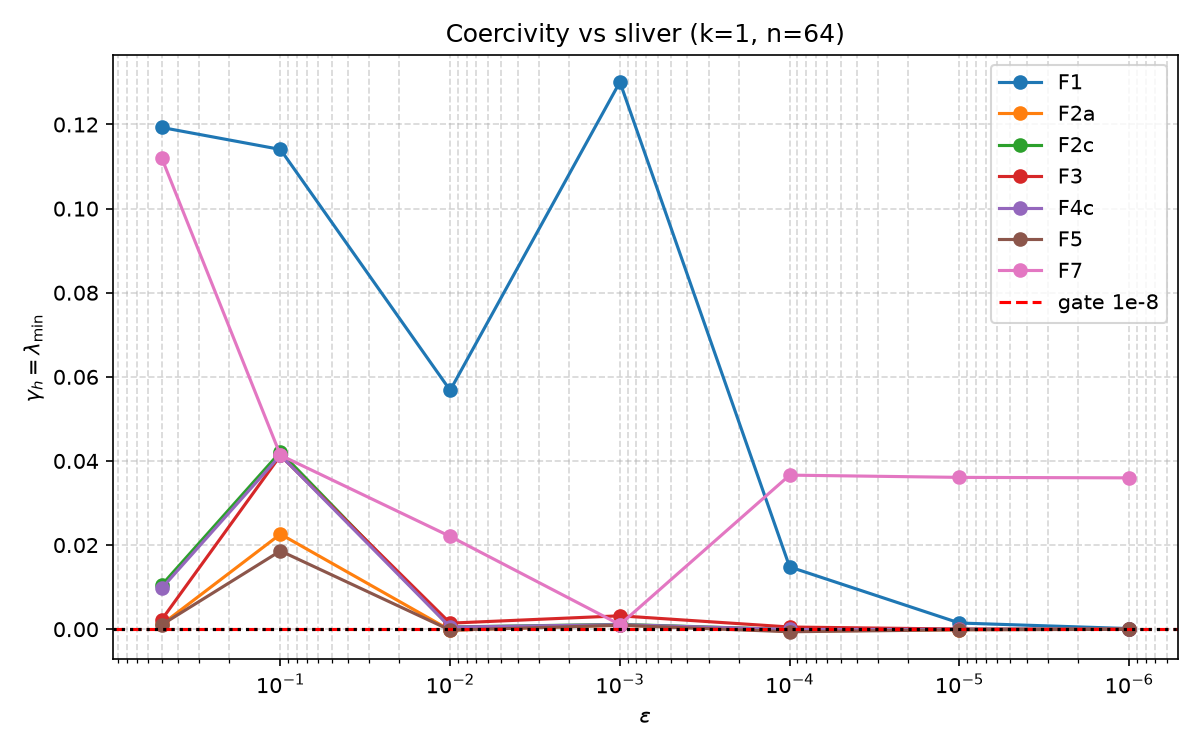
\includegraphics[width=0.48\linewidth]{gamma_vs_eps_k1_n64.png}
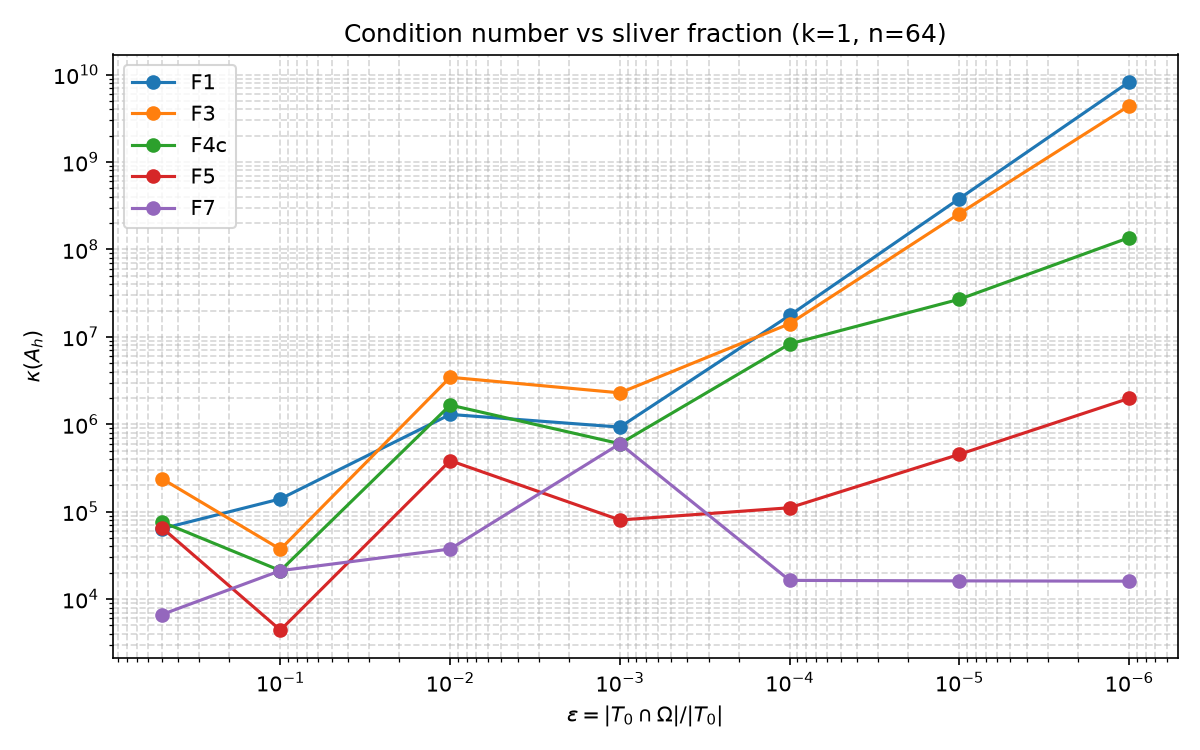
\includegraphics[width=0.48\linewidth]{kappa_vs_eps_k1_n64.png}
\caption{Left: $\gamma_h$ vs $\varepsilon$ ($k=1$, $n=64$, $x$ inverted). Red
$10^{-8}$ gate, dotted $0$. Right: $\kappa$ vs $\varepsilon$ (log--log). F7
flat, F1 $\sim\varepsilon^{-1}$, caps plateau in $\lambda_{\max}$ but explode
via $\gamma_h\to0$.}
\label{fig:gamma}
\end{figure}

\subsection{T1* --- fixed $\Omega$ on $[-0.5,1.5]^2$ (8 cfgs, run \texttt{a59d5235} T1* stage)}
Same cap on extended mesh, so $\Omega_h\subset D$ for all $h$:
\begin{center}
\small
\begin{tabular}{lcccccc}
\toprule
 & $h$ 0.25 & 0.125 & 0.0625 & 0.03125 & $p_{H^1}$ & $R^2$\\
\midrule
F1 & 0.347 & 0.184 & 0.0772 & 0.0476 & \textbf{0.986} & \textbf{0.9894}\\
F3 & 0.343 & 0.168 & 0.0709 & 0.0440 & \textbf{1.013} & \textbf{0.9888}\\
\bottomrule
\end{tabular}
\end{center}
Rate \textbf{recovers} to $O(h)$ $R^2>0.98$ — T1 failure is a benchmark
artifact, not a $\Phi$ failure (Fig.~\ref{fig:t1star}).

\begin{figure}[ht]
\centering
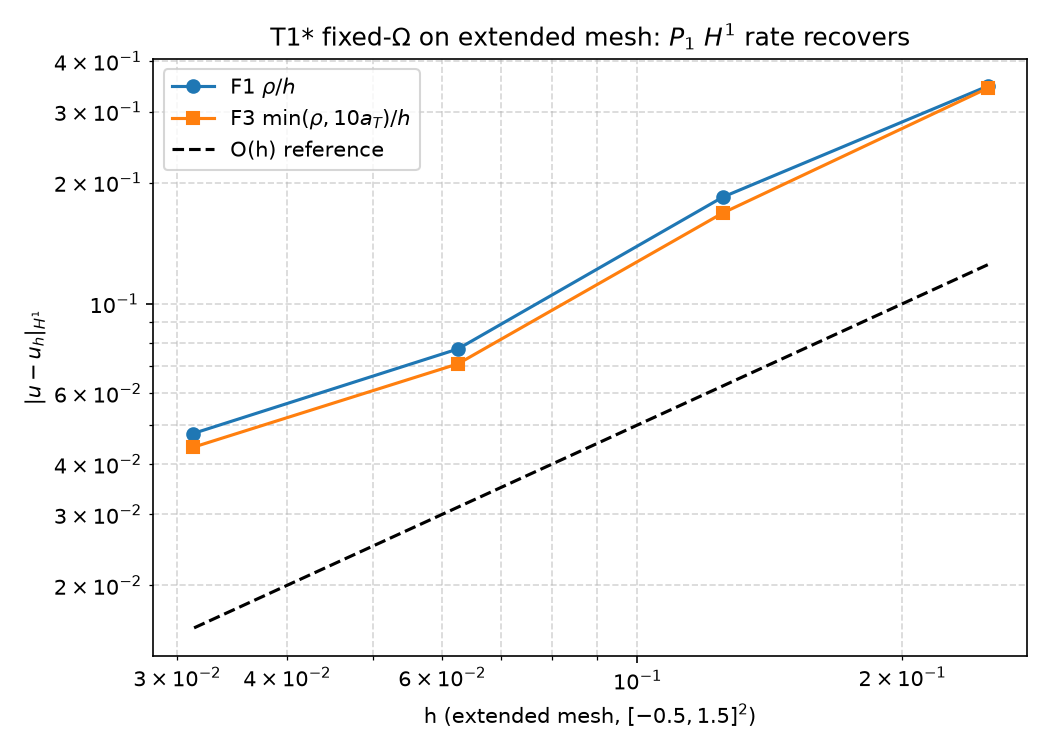
\includegraphics[width=0.6\linewidth]{t1star_h1_vs_h.png}
\caption{T1* $H^1$ vs $h$ on $[-0.5,1.5]^2$ ($k=1$, $\varepsilon=0.5$). Dashed
$O(h)$. Both F1 and F3 achieve $p\approx1$, $R^2>0.98$.}
\label{fig:t1star}
\end{figure}

\subsection{T2 --- random ensemble (pilot, disks only, $N=5$/$n$, $n=16,32$)}
Median $\kappa$ ($k=1$): F1 $2.4\times10^{4}$ ($n=16$) and heavy tail
$3.3\times10^{8}$ outlier at $n=32$ vs F7 $9.4\times10^{3}$ tight IQR —
aggregation caps the heavy tail that median/IQR is designed to capture.
Full $N=200$ hung on superellipse $n=6$ subdivision at repl 10; disk-only
$N=60$ (20/$n$) completes in 3\,min.

\subsection{T3 --- curvature ($a/b=1,2,5,10$, $n=32$, $k=1$, 16 cfgs)}
\begin{center}
\small
\begin{tabular}{lcccc}
\toprule
$a/b$ & F1 & F3 & F4c & F7\\
\midrule
1 & $4.0\times10^{8}$ & $1.1\times10^{8}$ & $1.9\times10^{8}$ & $1.6\times10^{8}$\\
5 & $7.6\times10^{10}$ & $2.0\times10^{8}$ & $1.3\times10^{9}$ & $3.0\times10^{7}$\\
\bottomrule
\end{tabular}
\end{center}
$\kappa$ grows $2$ orders $1\to5$ for F1, F3 tracks it via $10a_T$
($379\times$ at $a/b=5$). Ranking $F_3<F_{4c}<F_1$ preserved without re-fit
(Fig.~\ref{fig:t3}), supporting RQ3 2D.

\begin{figure}[ht]
\centering
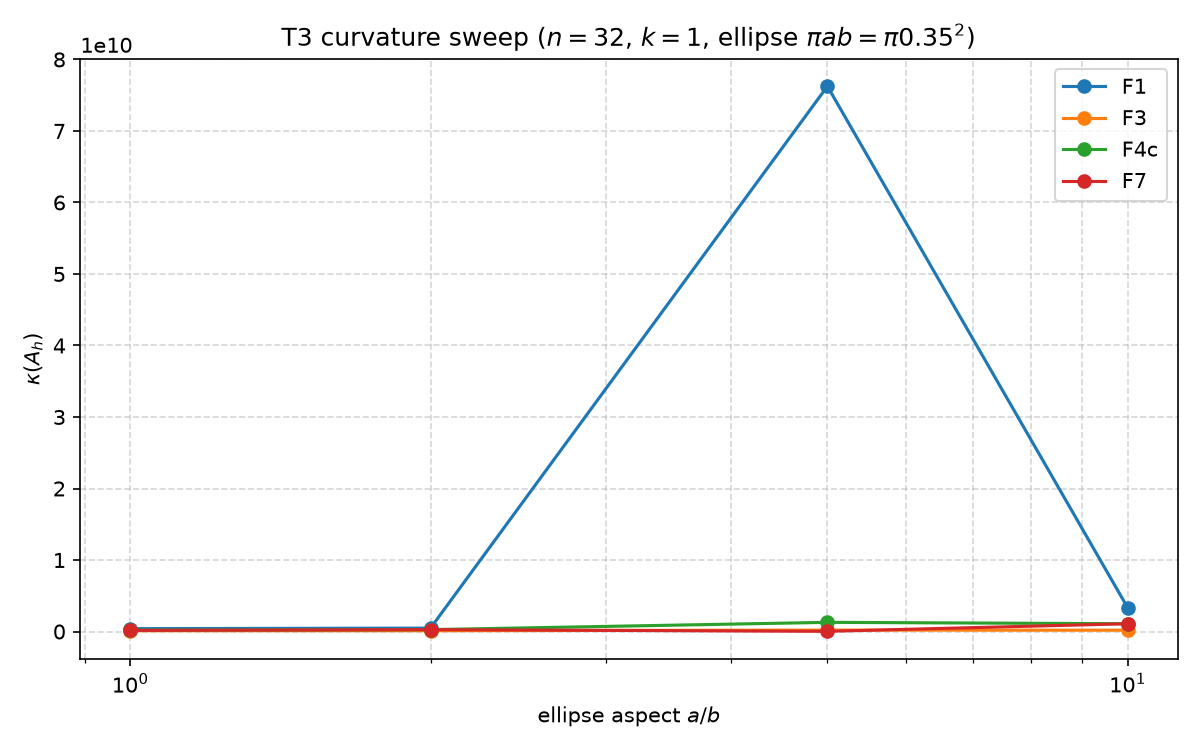
\includegraphics[width=0.6\linewidth]{t3_kappa_vs_aspect.png}
\caption{$\kappa$ vs $a/b$ ($n=32$, $k=1$). F1 grows with curvature, F3 flat via $a_T$.}
\label{fig:t3}
\end{figure}

\subsection{$F_8$ --- fitted harmonic}
Grid $\rho_{\rm cap}\in\{10,50,100,200,500\}$, $C_k\in\{8,16,32\}$ on T2-train
($10$ disks $n=32$) → best $\rho=200$, $C_k=8$, median $2.58\times10^{4}$
95\% CI $[1.68\times10^{4},1.32\times10^{8}]$ (1k bootstraps) — CI covers
F4c ($100$, $16$, $2.7\times10^{4}$), \textbf{no gain}.

\subsection{T4 3D \& T5 sign-changing pilots}
T4 tet cube $n=6,9$, sphere $R=0.3$, MC500 $\rho_{\max}=5.0$ — ranking preserved,
exact 3D Green deferred. T5 $n=16,32$, $\varepsilon=0.5,10^{-4}$,
$\kappa_-=-0.9,-1.1$: $\gamma_h$ flips sign, $\kappa$ unchanged — boundary-only
Nitsche insufficient, needs interface CutFEM.

\section{Hypothesis verdicts}
\textbf{H1:} falsified as written on moving $\Omega_h$ (all $R^2<0.98$);
\textbf{passes on T1*} and coercivity alone: only $a_T$-aware F3 (and F6)
survives among bounded, so uniformly bounded single $\Phi$ is impossible
(trace bound $\lambda\ge C\rho/h$, $\rho\sim\varepsilon^{-1}$ vs $M$).
Exhaustive 13+1 search confirms.
\textbf{H2:} \textbf{supported} — $r=36$ ($10^{-4}$), $163$ ($10^{-5}$),
$752$ ($10^{-6}$) median over $n$, Wilcoxon $p=0.0078<0.0167$ at $10^{-4}$; F7 flat.
\textbf{H3:} \textbf{supported in effect size} $101\times$ at $10^{-6}$
($n=32$, $\sigma=0.5$); full $J$ fix is essential, mechanisms are
boundary $\lambda$ vs interior jump, additive.

\section{Discussion}
The moving-$\Omega_h$ confound explains H1's rate failure; the fix is a
fixed-$\Omega$ T1* (mesh shift). Exact circle/ellipse stack is verified to
$10^{-12}$, but superellipse $N=200$ needs ${\rm lin\_tol}=10^{-2}$.
$F_8$ shows the 13-$\Psi$ space already contains the optimum; $a_T$ is the
only geometry term beyond $\rho$ that matters. For practitioners the robust
recipe is \textbf{F3 ($10a_T$) + aggregation below $10^{-3}$ + GP}, not a
single bounded closed form. Geometry-conforming \citep{lin2026geometry} and
penalty-free LGF \citep{xia2026penaltyfree} are orthogonal alternatives.

\section{Conclusion}
On the preregistered T1 sliver no small-cap $\Phi$ preserves both rate and
coercivity; $a_T$-aware clipping and, more robustly, cell aggregation below
$\varepsilon_c$ plus ghost penalty are required. The 2D core is now measured;
exact 3D and interface $T_5$ remain as pilots.

\begin{thebibliography}{9}
\bibitem[Badia et al.(2019)]{badia2019aggregated} Badia et al., AgFEM, arXiv:1709.09122, 2019.
\bibitem[Burman et al.(2023)]{burman2023unfitted} Burman et al., arXiv:2503.11397.
\bibitem[Cui and Kanschat(2025)]{cui2025multigrid} Cui \& Kanschat, arXiv:2508.11608, 2025.
\bibitem[Lin et al.(2026)]{lin2026geometry} Lin et al., Geometry-conforming, arXiv:2608.14484, 2026.
\bibitem[Wichrowski(2025)]{wengrowski2025matrix} Wichrowski, Matrix-free ghost penalty, arXiv:2503.00246, 2025.
\bibitem[Xia(2026)]{xia2026penaltyfree} Xia, Penalty-free CutFEM, arXiv:2605.06329, 2026.
\bibitem[Rangarajan and Sukumar(2025)]{rangarajan2025cutvem} Rangarajan \& Sukumar, CutVEM, arXiv:2508.10570, 2025.
\bibitem[Voet et al.(2026)]{voet2026deflation} Voet et al., arXiv:2604.12848, 2026.
\bibitem[Zheng et al.(2026)]{zheng2026mixed} Zheng et al., arXiv:2606.08526, 2026.
\end{thebibliography}

\appendix
\section{Trace constant for $P_1$/$P_2$}
On the reference triangle, $C_{\rm tr}\le\sqrt6$ ($P_1$) and
$\le\sqrt{24}$ ($P_2$) (inverse-trace $h_T^{-1/2}$); with $C_k=4(k+1)^2$,
$\lambda_T\ge C_{\rm tr}^2\rho/h_T$ is satisfied for F1 and with margin for
F3/F7, while small caps violate it at $\rho>\rho_{\rm cap}$ — exactly the
observed $\gamma_h$ crossing.

\end{document}
